\documentclass{article}%
\usepackage[T1]{fontenc}%
\usepackage[utf8]{inputenc}%
\usepackage{lmodern}%
\usepackage{textcomp}%
\usepackage{lastpage}%
\usepackage{xcolor}%
\usepackage{tikz}%
\usepackage[left=0.5in, right=0.5in, top=1in, bottom=1in]{geometry}%
%
\definecolor{P0}{HTML}{ddf590}%
\definecolor{P1}{HTML}{90f5f0}%
\definecolor{P2}{HTML}{90d0f5}%
\definecolor{P3}{HTML}{e190f5}%
%
\begin{document}%
\normalsize%
\section{Priority Scheduling}%
\label{sec:PriorityScheduling}%

        \section*{Introduction}
        Priority scheduling is a scheduling algorithm that schedules processes according to the priority assigned to each process. Higher priority processes are executed before lower priority processes; Processes with the same priority are executed in the "execution in order of arrival" method. Also, priority scheduling is a non-preemptive paradigm.
        %
\subsection{Time 0: Process P1}%
\label{subsec:Time0ProcessP1}%


\begin{figure}[h!]%
\centering%
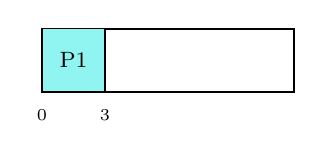
\begin{tikzpicture}%
\draw[thick] (0,0) rectangle (3.200000, 0.800000);%
\node[draw, minimum width=0.800000cm, minimum height=0.800000cm, text centered, fill=P1, font=\fontsize{8}{9}\selectfont] at (0.400000, 0.400000) {P1};%
\node[font=\fontsize{6}{8}\selectfont] at (0.000000, -0.3) {0};%
\node[font=\fontsize{6}{8}\selectfont] at (0.800000, -0.3) {3};%
\end{tikzpicture}%
\end{figure}

%
\subsection{Time 3: Process P3}%
\label{subsec:Time3ProcessP3}%


\begin{figure}[h!]%
\centering%
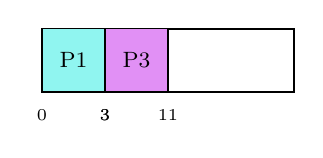
\begin{tikzpicture}%
\draw[thick] (0,0) rectangle (3.200000, 0.800000);%
\node[draw, minimum width=0.800000cm, minimum height=0.800000cm, text centered, fill=P1, font=\fontsize{8}{9}\selectfont] at (0.400000, 0.400000) {P1};%
\node[font=\fontsize{6}{8}\selectfont] at (0.000000, -0.3) {0};%
\node[font=\fontsize{6}{8}\selectfont] at (0.800000, -0.3) {3};%
\node[draw, minimum width=0.800000cm, minimum height=0.800000cm, text centered, fill=P3, font=\fontsize{8}{9}\selectfont] at (1.200000, 0.400000) {P3};%
\node[font=\fontsize{6}{8}\selectfont] at (0.800000, -0.3) {3};%
\node[font=\fontsize{6}{8}\selectfont] at (1.600000, -0.3) {11};%
\end{tikzpicture}%
\end{figure}

%
\subsection{Time 11: Process P2}%
\label{subsec:Time11ProcessP2}%


\begin{figure}[h!]%
\centering%
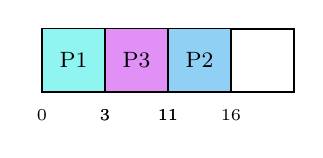
\begin{tikzpicture}%
\draw[thick] (0,0) rectangle (3.200000, 0.800000);%
\node[draw, minimum width=0.800000cm, minimum height=0.800000cm, text centered, fill=P1, font=\fontsize{8}{9}\selectfont] at (0.400000, 0.400000) {P1};%
\node[font=\fontsize{6}{8}\selectfont] at (0.000000, -0.3) {0};%
\node[font=\fontsize{6}{8}\selectfont] at (0.800000, -0.3) {3};%
\node[draw, minimum width=0.800000cm, minimum height=0.800000cm, text centered, fill=P3, font=\fontsize{8}{9}\selectfont] at (1.200000, 0.400000) {P3};%
\node[font=\fontsize{6}{8}\selectfont] at (0.800000, -0.3) {3};%
\node[font=\fontsize{6}{8}\selectfont] at (1.600000, -0.3) {11};%
\node[draw, minimum width=0.800000cm, minimum height=0.800000cm, text centered, fill=P2, font=\fontsize{8}{9}\selectfont] at (2.000000, 0.400000) {P2};%
\node[font=\fontsize{6}{8}\selectfont] at (1.600000, -0.3) {11};%
\node[font=\fontsize{6}{8}\selectfont] at (2.400000, -0.3) {16};%
\end{tikzpicture}%
\end{figure}

%
\subsection{Time 16: Process P0}%
\label{subsec:Time16ProcessP0}%


\begin{figure}[h!]%
\centering%
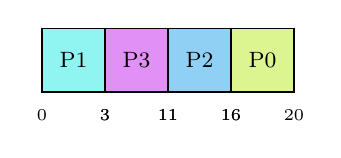
\begin{tikzpicture}%
\draw[thick] (0,0) rectangle (3.200000, 0.800000);%
\node[draw, minimum width=0.800000cm, minimum height=0.800000cm, text centered, fill=P1, font=\fontsize{8}{9}\selectfont] at (0.400000, 0.400000) {P1};%
\node[font=\fontsize{6}{8}\selectfont] at (0.000000, -0.3) {0};%
\node[font=\fontsize{6}{8}\selectfont] at (0.800000, -0.3) {3};%
\node[draw, minimum width=0.800000cm, minimum height=0.800000cm, text centered, fill=P3, font=\fontsize{8}{9}\selectfont] at (1.200000, 0.400000) {P3};%
\node[font=\fontsize{6}{8}\selectfont] at (0.800000, -0.3) {3};%
\node[font=\fontsize{6}{8}\selectfont] at (1.600000, -0.3) {11};%
\node[draw, minimum width=0.800000cm, minimum height=0.800000cm, text centered, fill=P2, font=\fontsize{8}{9}\selectfont] at (2.000000, 0.400000) {P2};%
\node[font=\fontsize{6}{8}\selectfont] at (1.600000, -0.3) {11};%
\node[font=\fontsize{6}{8}\selectfont] at (2.400000, -0.3) {16};%
\node[draw, minimum width=0.800000cm, minimum height=0.800000cm, text centered, fill=P0, font=\fontsize{8}{9}\selectfont] at (2.800000, 0.400000) {P0};%
\node[font=\fontsize{6}{8}\selectfont] at (2.400000, -0.3) {16};%
\node[font=\fontsize{6}{8}\selectfont] at (3.200000, -0.3) {20};%
\end{tikzpicture}%
\end{figure}

%
\subsection{Final Process Table}%
\label{subsec:FinalProcessTable}%
\begin{tabular}{|c|c|c|c|c|}%
\hline%
\textbf{Process}&\textbf{Arrival Time}&\textbf{Burst Time}&\textbf{Priority}&\textbf{Service Time}\\%
\hline%
P0&0&4&1&16\\%
\hline%
P1&0&3&2&0\\%
\hline%
P2&1&5&5&11\\%
\hline%
P3&1&8&6&3\\%
\hline%
\end{tabular}

%
\subsection{Execution Order}%
\label{subsec:ExecutionOrder}%


\begin{figure}[h!]%
\centering%
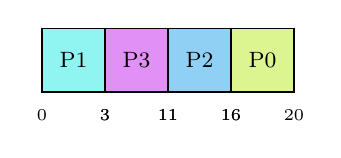
\begin{tikzpicture}%
\draw[thick] (0,0) rectangle (3.200000, 0.800000);%
\node[draw, minimum width=0.800000cm, minimum height=0.800000cm, text centered, font=\fontsize{8}{9}\selectfont, fill=P1] at (0.400000, 0.400000) {P1};%
\node[font=\fontsize{6}{8}\selectfont] at (0.000000, -0.3) {0};%
\node[font=\fontsize{6}{8}\selectfont] at (0.800000, -0.3) {3};%
\node[draw, minimum width=0.800000cm, minimum height=0.800000cm, text centered, font=\fontsize{8}{9}\selectfont, fill=P3] at (1.200000, 0.400000) {P3};%
\node[font=\fontsize{6}{8}\selectfont] at (0.800000, -0.3) {3};%
\node[font=\fontsize{6}{8}\selectfont] at (1.600000, -0.3) {11};%
\node[draw, minimum width=0.800000cm, minimum height=0.800000cm, text centered, font=\fontsize{8}{9}\selectfont, fill=P2] at (2.000000, 0.400000) {P2};%
\node[font=\fontsize{6}{8}\selectfont] at (1.600000, -0.3) {11};%
\node[font=\fontsize{6}{8}\selectfont] at (2.400000, -0.3) {16};%
\node[draw, minimum width=0.800000cm, minimum height=0.800000cm, text centered, font=\fontsize{8}{9}\selectfont, fill=P0] at (2.800000, 0.400000) {P0};%
\node[font=\fontsize{6}{8}\selectfont] at (2.400000, -0.3) {16};%
\node[font=\fontsize{6}{8}\selectfont] at (3.200000, -0.3) {20};%
\end{tikzpicture}%
\end{figure}

%
\end{document}